\documentclass[a4paper,11pt]{exam}
%\printanswers % pour imprimer les réponses (corrigé)
\noprintanswers % Pour ne pas imprimer les réponses (énoncé)
\addpoints % Pour compter les points
% \noaddpoints % pour ne pas compter les points
%\qformat{\textbf{\thequestion ) } }
\qformat{\textbf{\thequestion )} \textit{(\thepoints)} \\  } % Pour définir le style des questions (facultatif)
\usepackage{color} % définit une nouvelle couleur
\shadedsolutions % définit le style des réponses
% \framedsolutions % définit le style des réponses
\definecolor{SolutionColor}{rgb}{0.8,0.9,1} % bleu ciel
\renewcommand{\solutiontitle}{\noindent\textbf{Solution:}\par\noindent} % Définit le titre des solutions




\makeatletter

\def\maketitle{{\centering%
	\par{\huge\textbf{\@title}}%
	\par{\@date}%
	\par}}

\makeatother

\lhead{NOM Pr\'enom :}
\rhead{\textbf{Les r\'eponses doivent \^etre justifi\'ees}}
\cfoot{\thepage / \pageref{LastPage}}


%\usepackage{../../pas-math}
%\usepackage{../../moncours}


%\usepackage{pas-cours}
%-------------------------------------------------------------------------------
%          -Packages nécessaires pour écrire en Français et en UTF8-
%-------------------------------------------------------------------------------
\usepackage[utf8]{inputenc}
\usepackage[frenchb]{babel}
\usepackage[T1]{fontenc}
\usepackage{lmodern}
\usepackage{textcomp}



%-------------------------------------------------------------------------------

%-------------------------------------------------------------------------------
%                          -Outils de mise en forme-
%-------------------------------------------------------------------------------
\usepackage{hyperref}
\hypersetup{pdfstartview=XYZ}
%\usepackage{enumerate}
\usepackage{graphicx}
\usepackage{multicol}
\usepackage{tabularx}
\usepackage{multirow}


\usepackage{anysize} %%pour pouvoir mettre les marges qu'on veut
%\marginsize{2.5cm}{2.5cm}{2.5cm}{2.5cm}

\usepackage{indentfirst} %%pour que les premier paragraphes soient aussi indentés
\usepackage{verbatim}
\usepackage{enumitem}
\usepackage[usenames,dvipsnames,svgnames,table]{xcolor}

\usepackage{variations}

%-------------------------------------------------------------------------------


%-------------------------------------------------------------------------------
%                  -Nécessaires pour écrire des mathématiques-
%-------------------------------------------------------------------------------
\usepackage{amsfonts}
\usepackage{amssymb}
\usepackage{amsmath}
\usepackage{amsthm}
\usepackage{tikz}
\usepackage{xlop}
%-------------------------------------------------------------------------------



%-------------------------------------------------------------------------------


%-------------------------------------------------------------------------------
%                    - Mise en forme avancée
%-------------------------------------------------------------------------------

\usepackage{ifthen}
\usepackage{ifmtarg}


\newcommand{\ifTrue}[2]{\ifthenelse{\equal{#1}{true}}{#2}{$\qquad \qquad$}}

%-------------------------------------------------------------------------------

%-------------------------------------------------------------------------------
%                     -Mise en forme d'exercices-
%-------------------------------------------------------------------------------
%\newtheoremstyle{exostyle}
%{\topsep}% espace avant
%{\topsep}% espace apres
%{}% Police utilisee par le style de thm
%{}% Indentation (vide = aucune, \parindent = indentation paragraphe)
%{\bfseries}% Police du titre de thm
%{.}% Signe de ponctuation apres le titre du thm
%{ }% Espace apres le titre du thm (\newline = linebreak)
%{\thmname{#1}\thmnumber{ #2}\thmnote{. \normalfont{\textit{#3}}}}% composants du titre du thm : \thmname = nom du thm, \thmnumber = numéro du thm, \thmnote = sous-titre du thm

%\theoremstyle{exostyle}
%\newtheorem{exercice}{Exercice}
%
%\newenvironment{questions}{
%\begin{enumerate}[\hspace{12pt}\bfseries\itshape a.]}{\end{enumerate}
%} %mettre un 1 à la place du a si on veut des numéros au lieu de lettres pour les questions 
%-------------------------------------------------------------------------------

%-------------------------------------------------------------------------------
%                    - Mise en forme de tableaux -
%-------------------------------------------------------------------------------

\renewcommand{\arraystretch}{1.7}

\setlength{\tabcolsep}{1.2cm}

%-------------------------------------------------------------------------------



%-------------------------------------------------------------------------------
%                    - Racourcis d'écriture -
%-------------------------------------------------------------------------------

% Angles orientés (couples de vecteurs)
\newcommand{\aopp}[2]{(\vec{#1}, \vec{#2})} %Les deuc vecteurs sont positifs
\newcommand{\aopn}[2]{(\vec{#1}, -\vec{#2})} %Le second vecteur est négatif
\newcommand{\aonp}[2]{(-\vec{#1}, \vec{#2})} %Le premier vecteur est négatif
\newcommand{\aonn}[2]{(-\vec{#1}, -\vec{#2})} %Les deux vecteurs sont négatifs

%Ensembles mathématiques
\newcommand{\naturels}{\mathbb{N}} %Nombres naturels
\newcommand{\relatifs}{\mathbb{Z}} %Nombres relatifs
\newcommand{\rationnels}{\mathbb{Q}} %Nombres rationnels
\newcommand{\reels}{\mathbb{R}} %Nombres réels
\newcommand{\complexes}{\mathbb{C}} %Nombres complexes


%Intégration des parenthèses aux cosinus
\newcommand{\cosP}[1]{\cos\left(#1\right)}
\newcommand{\sinP}[1]{\sin\left(#1\right)}


%Probas stats
\newcommand{\stat}{statistique}
\newcommand{\stats}{statistiques}
%-------------------------------------------------------------------------------

%-------------------------------------------------------------------------------
%                    - Mise en page -
%-------------------------------------------------------------------------------

\newcommand{\twoCol}[1]{\begin{multicols}{2}#1\end{multicols}}


\setenumerate[1]{font=\bfseries,label=\textit{\alph*})}
\setenumerate[2]{font=\bfseries,label=\arabic*)}


%-------------------------------------------------------------------------------
%                    - Elements cours -
%-------------------------------------------------------------------------------




\usepackage{tabu}

%\usepackage{fullpage}
\author{\ }
\date{27 Février 2018}
\title{$T^{le}$ $ST_2S$ : DS num\'ero 3 (2)}


\begin{document}
%	\usepackage{fancyhdr}
%	
%	\pagestyle{fancy}
%	\fancyhf{}
	%\rhead{Share\LaTeX}

	\maketitle





\section{Salariés d'une entreprise pharmaceutique}

Le tableau suivant donne la répartition des \num{1300} salariés d'une entreprise du secteur pharmaceutique en fonction de leur salaire moyen (exprimé en euros) et de leur sexe.

\begin{center}
	\begin{tabular}{|c|c|c|}
		\hline
		& Hommes & Femmes \\ \hline
		{[}1000 ; 1500{[}  & 440    & 400    \\ \hline
		{[}1500 ; 2000{[}  & 200    & 180    \\ \hline
		{[}2000  ; 2500{[} & 50     & 15     \\ \hline
		{[}2500 ; 3000{[}  & 10     & 5      \\ \hline
	\end{tabular}
\end{center}

\emph{Dans cet exercice, tous les résultats seront arrondis à $10^{-2} $. Dans chaque classe, on admet que la populations est au centre.}


\begin{questions}
	\question[3]\label{q:1} Déterminer :
		\begin{parts}
			\part[1] le salaire moyen de hommes ;
			\part[1] le salaire moyen des femmes ;
			\part[1] le salaire moyen de l'ensemble des salariés de l'entreprise.
		\end{parts} 
	
	\question[3] On note : 
	$H$ la sous population des hommes parmi les salariés, et $C$ la sous-population des cadres (les salariés ayant un salaire compris entre \num{2000} et \num{2500} euros).
	
	\begin{parts}
		\part[1] Calculer les fréquences respectives des, notées $f(H)$, $f(C)$, $f(H \cap C)$, des sous-populations $H$, $C$ et $H \cap C$ dans l'ensemble des salariés de l'entreprise.
		
		\part[1] \`A l'aide du tableau et des résultats obtenus au \ref{q:1} calculer la fréquence de la sous-population des cadres dans la sous-population des hommes. Cette fréquence appelée <<fréquence de $C$ sachant $H$>> est notée $f_H(C)$.
		
		\part[1] vérifier que $f_H(C) = \dfrac{f(H \cap C)}{f(H)}$
	\end{parts}
\end{questions}

%\newpage 

%\section{Taux d'évolution, ajustement affine}

Le tableau suivant donne la consommation de soins et biens médicaux (CSBM) en France de 2001 à 2008.

\begin{questions}
	\question[] Calculer le taux d'évolution de la CSBM entre 2001 et 2008. Arrondir à \num{0.01} \%.
	
	\question[] Calculer le montant des dépenses de médicaments en 2008 sachant qu'elles représentaient \num{24.47}  \% de la CSBM. Arrondir au milliard.
	
	\question[] Représenter par un nuage de points $M_i(x_i, y_i)$ la série statistique correspondant aux données du tableau. ON utilisera un repère orthogonal du plan tel que :
	\begin{itemize}
		\item 2 cm représentent une année sur l'axe des abscisses,
		
		\item 2 cm représentent 10 milliards d'euros sur l'axe des ordonnées (cet axe sera gradué de 100 à 200).
		
	\end{itemize}

	\question[] 
		\begin{parts}
			\part[] Calculer les coordonnées du point moyen G du nuage. Placer le point G sur le graphique.
			
			\part[] Soit $\delta$ la droite de coefficient directeur \num{6.7} passant par le point G ; déterminer une équation de la droite $\delta$. Tracer la droite $\delta$ sur le graphique.
			
			\part[] Cette droite vous paraît-elle représenter un bon ajustement du nuage de points ? Pourquoi ?
		\end{parts}
	
		\question[] On admet que l'ajustement réalisé par la droite $\delta$ est valable jusqu'en 2010. Déterminer graphiquement :
			\begin{parts}
				\part[]  Une estimation de la CSBM en 2010.
				\part[] l'année au cours de laquelle la CSBM a dépassé 175 milliards d'euros.
			\end{parts}
		
		\question[] justifier par le calcul les résultats de la question précédente.
\end{questions}

%\newpage 

\section{La tension artérielle en fonction de l'âge}

Le tableau suivant donne, dans une population féminine, la moyenne de la tension artérielle maximale en fonction de l'âge.

\begin{questions}
	\question[] Représenter graphiquement le nuage de points de coordonnées $(x,y)$ de cette série dans un repère orthogonal. 
	On graduera l'axe des abscisses à partir de 36 et l'axe des ordonnées à partir de 11.
	De plus on prendra pour unités graphiques : \num{0.5} cm pour une année et 2 cm pour une unité de tension.
	
	\question[] H désigne le point moyen des 3 premiers points du nuage et K celui des 3 derniers points.
		\begin{parts}
			\part[] Déterminer les coordonnées des points H et K.
			\part[] Tracer la droite (HK).
			\part[] Vérifier que la droite (HK) a pour équation :
				\begin{equation*}
					y = \frac{1}{9}x + \frac{25}{3}.
				\end{equation*}
		\end{parts}
	
	\question[] On admet que la droite (HK) constitue un ajustement convenable du nuage de points précédent.
	\begin{parts}
		\part[] Déterminer graphiquement, en faisant apparaître les traits de construction utiles, la tension artérielle maximale prévisible pour une personne de 70 ans.
		\part[] Vérifier le résultat précédent par le calcul en utilisant l'équation de la droite (HK).
	\end{parts}
\end{questions}

\newpage 

%\section{Un vrai-faux (6 points)}

Répondez par VRAI ou FAUX aux affirmations suivantes. Une justification est demandée lorsque la réponse est FAUX, aucune justification n'est demandée lorsque la réponse est VRAI.

\begin{questions}
	\question[1] Pour une série ordonnée comptant 512 nombres, la médiane n'existe pas car 512 est pair.
	
	\question[1] En France, le salaire mensuel moyen s'élève à \num{2500} € et le salaire mensuel médian s'élève à \num{1600} €. Plus de 50 \% des salariés gagnent moins de \num{2500} € par mois.
	
	\question[1] Le couple médiane et écart interquartile est peu sensible aux valeurs extrêmes de la série statistique.
	
	\question[1] La moyenne rend compte de la dispersion de la série statistique.
	
	\question[1] Si une série statistique compte 10 valeurs, les quartiles sont toujours des valeurs de la série.
	
	\question[1] On donne la série : 1 ; 2 ; 3 ; 4 ; 4 ; 4 ; 5 ; 8 ; 9 ; 10. L'écart interquartille est 5.
\end{questions}

%\section{Implantation d'éoliennes \textit{(12,5 points)}}

Les parties \ref{part:site_M} et \ref{part:site_F} sont indépendantes.

Après étude, les autorités d'une ile isolée ont décidé d'installer une éolienne pour répondre aux besoins énergétiques de leur communauté. L'éolienne choisie fonctionne lorsque le vent atteint au moins 8 n\oe uds et il faut l'arrêter lorsque le vent atteint ou dépasse les 48 n\oe uds. 

\subsection{\'Etude des vitesses du vent sur le site M \textit{(7 points)}}\label{part:site_M}

Les autorités décident de mesurer pendant un mois, à l'aide d'un anémomètre, la vitesse du vent sur le site M, au sommet d'une montagne. Une mesure est effectuée chaque jour.

Les résultats obtenus sont présentés dans la tableau de la figure \ref{tab:site_M} (le mois comporte 30 jours) :

\begin{figure}[h]
	\begin{center}
		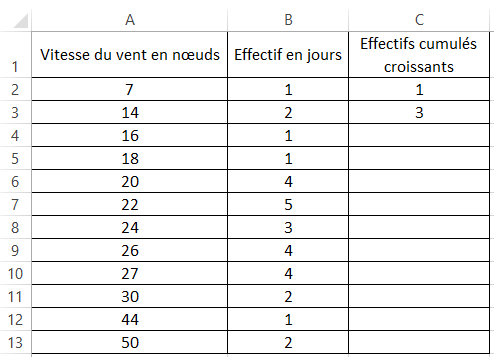
\includegraphics[scale=0.8]{eoliennes2}
	\end{center}
\caption{\'Etude de la vitesse du vent sur le site M}
\label{tab:site_M}
\end{figure}

On peut y lire que la vitesse de 22 n\oe uds a été mesurée 5 jours.

\begin{questions}
	\question[3]
		\begin{parts}
			\part[1] Compléter le tableau.
			
			\part[1] Donner une formule à placer en \textbf{\texttt{C3}} permettant, par recopie vers le bas, de calculer les effectifs cumulés croissants des jours du mois étudié.
			
			\part[1] Calculer le pourcentage des jours du mois étudié où l'éolienne ne produirait pas d'électricité. 
		\end{parts}
	
	
	\question[2] Déterminer l'étendue, la médiane, les quartiles et l'écart interquartile de cette série statistique.
	
	\question[1] On appelle premier décile (noté $D_1$) la plus petite valeur de la vitesse du vent, telle qu'au moins 10 \% des valeurs de la série sont inférieures ou égales à $D_1$. On appelle neuvième décile (noté $D_9$) la plus petite valeur, telle qu'au moins 90 \% des valeurs de la série lui sont inférieures ou égales.
	\begin{parts}
		\part[\half] Expliquer pourquoi $D_1$ = 14.
		\part[\half] Déterminer $D_9$.
	\end{parts} 
	
\end{questions}

\subsection{\'Etude des vitesses du vent sur le site F \textit{(2 points)}}\label{part:site_F}

Un emplacement sur une falaise, appelé site F, a également été retenu. Le même mois que le site M, on a mesuré les vitesses du vent sur le site F.

La série des mesures effectuée est dans le diagramme en boite de la figure \ref{fig:comparaison}. Les extrémités du diagramme correspondent aux premiers et neuvième déciles.

\begin{questions}
	
	\question[1] Lire sur le graphique les quartiles de cette nouvelle série.
	
	\question[1] Calculer l'écart interquartile.
\end{questions}

\begin{figure}[h]
	\begin{center}
		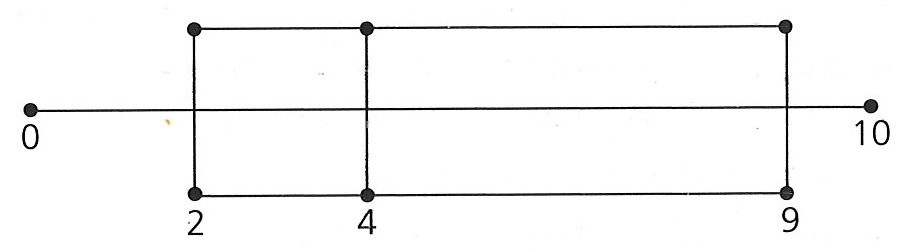
\includegraphics[scale=1.2]{moustache}
	\end{center}
	\caption{Coparaison de la vitesse du vent sur les deux sites}
	\label{fig:comparaison}
\end{figure}

\subsection{Comparaison des sites \textit{(3,5 points)}}\label{part:comp}

\begin{questions}
	\question[1\half] Représenter au-dessous du diagramme en boite fourni figure \ref{fig:comparaison}, celui de la série correspondant au site M. Prendre comme extrémités les premier et neuvième déciles.
	
	\question[2] En comparant les diagrammes, sachant qu'une éolienne a un rendement optimal aux alentours de 23 n\oe uds, quel site paraît le plsu intéressant pour l'installation de l'éolienne ? Argumenter la réponse. 
\end{questions}

\label{LastPage}
	

\end{document}